\section{Kotlin vs. Java}
\subsection{Sintaxis}
\begin{frame}{Sintaxis}{}
    \begin{figure}[h]
    \centering
    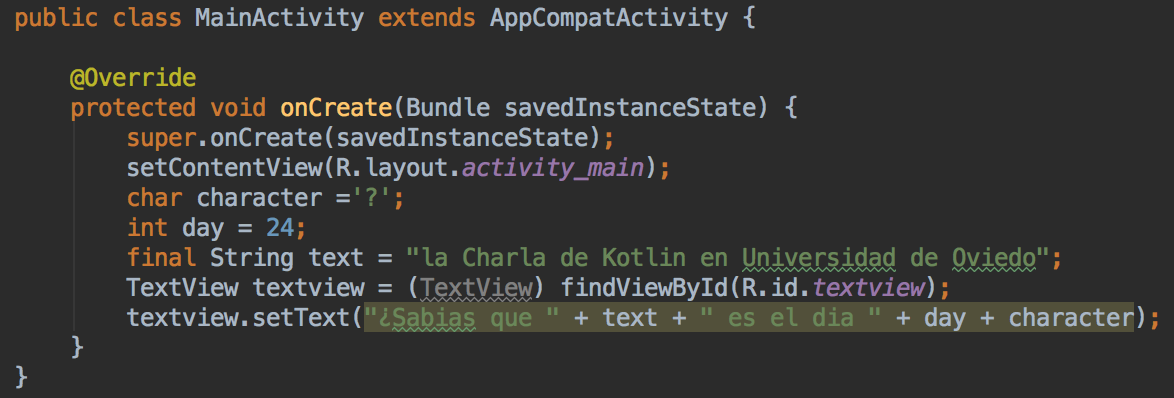
\includegraphics[width=\textwidth]{images/kotlin_vs_java/java_basic}
    \vspace{0pt}
    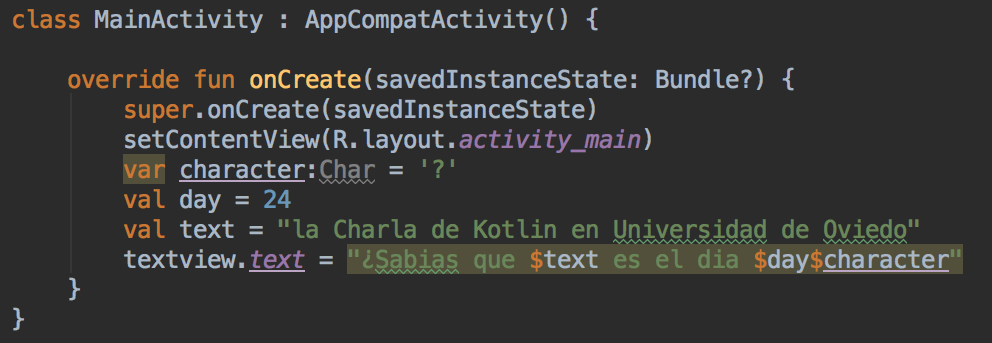
\includegraphics[width=\textwidth]{images/kotlin_vs_java/kotlin_basic}
    \end{figure}
\end{frame}
%%%%%%%%%%%%%%%%

\begin{frame}{Sintaxis}{Punto y coma opcional}
    \begin{figure}[h]
    \centering
    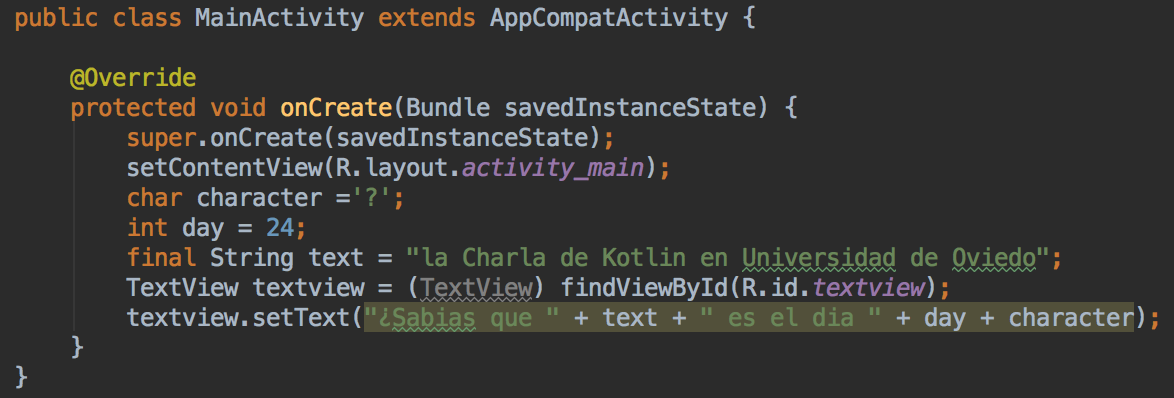
\includegraphics[width=\textwidth]{images/kotlin_vs_java/java_basic}
    \vspace{0pt}
    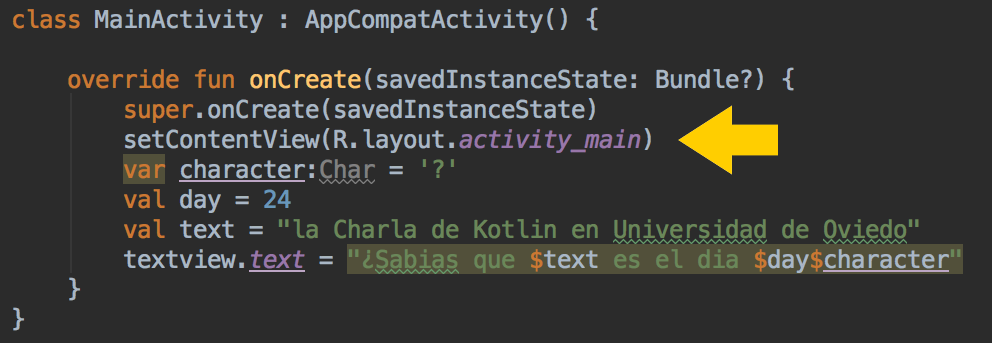
\includegraphics[width=\textwidth]{images/kotlin_vs_java/kotlin_semicolon}
    \end{figure}
\end{frame}
%%%%%%%%%%%%%%%%

\begin{frame}{Sintaxis}{fun}
    \begin{figure}[h]
    \centering
    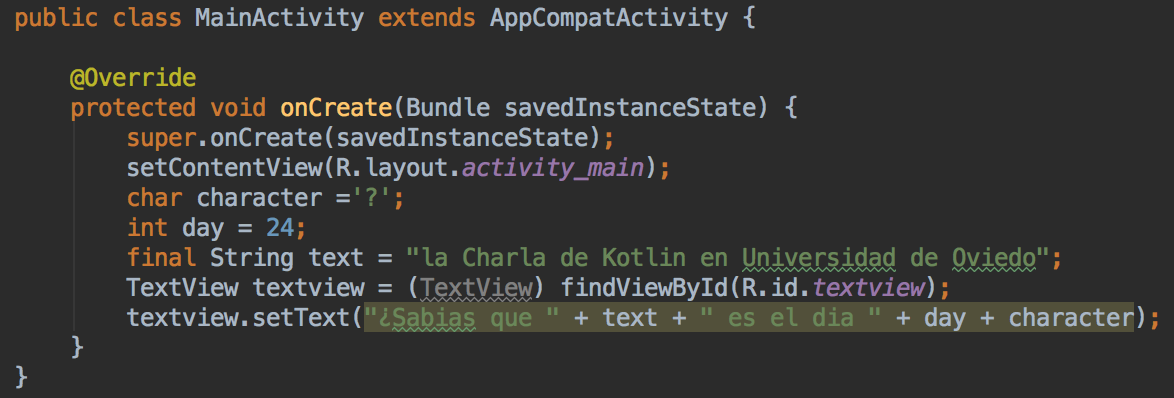
\includegraphics[width=\textwidth]{images/kotlin_vs_java/java_basic}
    \vspace{0pt}
    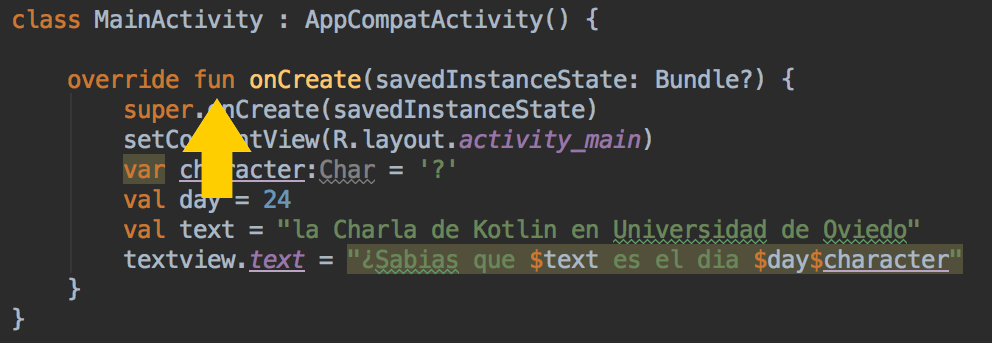
\includegraphics[width=\textwidth]{images/kotlin_vs_java/kotlin_fun}
    \end{figure}
\end{frame}
%%%%%%%%%%%%%%%%

\begin{frame}{Sintaxis}{Todo es un objeto. No más tipos primitivos}
    \begin{figure}[h]
    \centering
    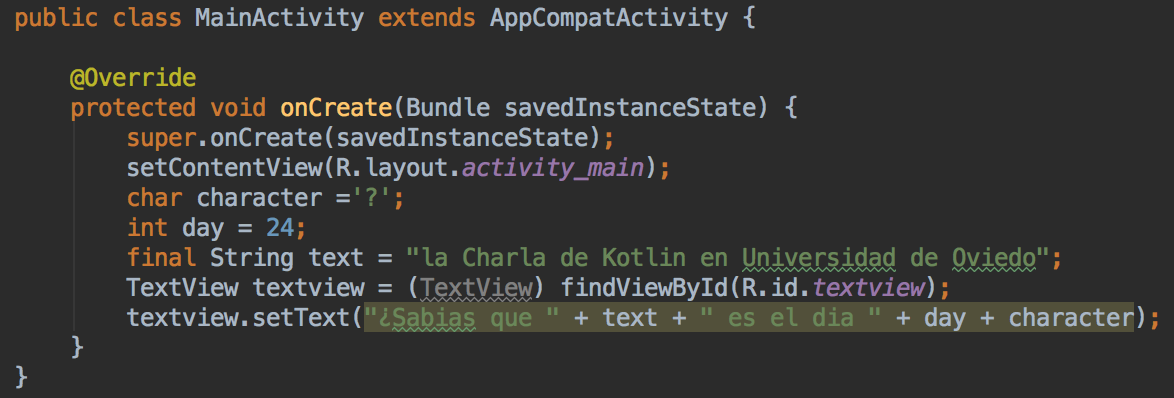
\includegraphics[width=\textwidth]{images/kotlin_vs_java/java_basic}
    \vspace{0pt}
    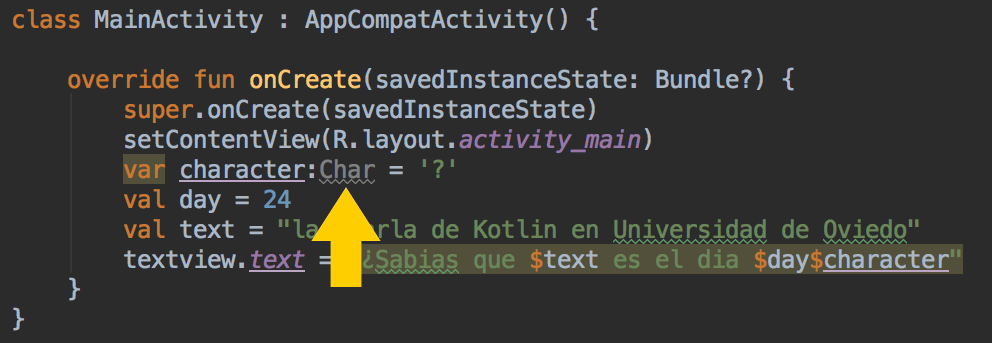
\includegraphics[width=\textwidth]{images/kotlin_vs_java/kotlin_primitives}
    \end{figure}
\end{frame}
%%%%%%%%%%%%%%%%

\begin{frame}{Sintaxis}{val \& var}
    \begin{figure}[h]
    \centering
    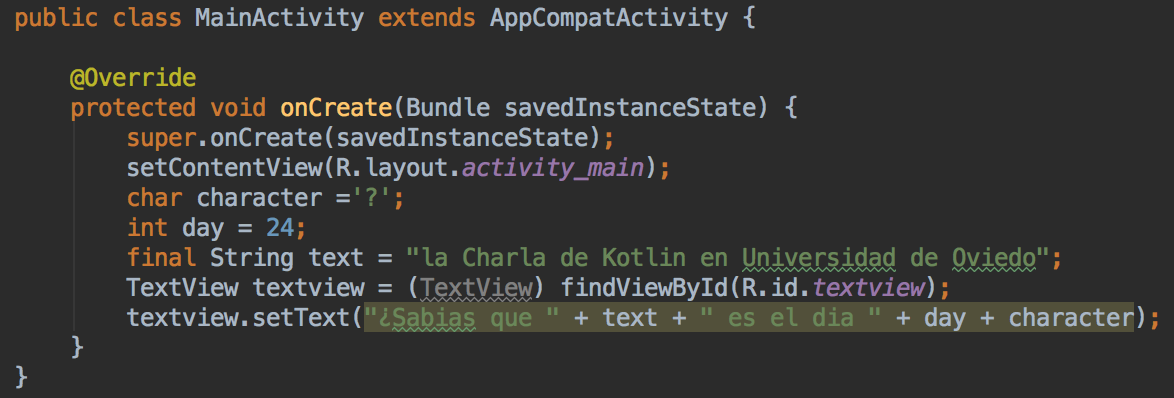
\includegraphics[width=\textwidth]{images/kotlin_vs_java/java_basic}
    \vspace{0pt}
    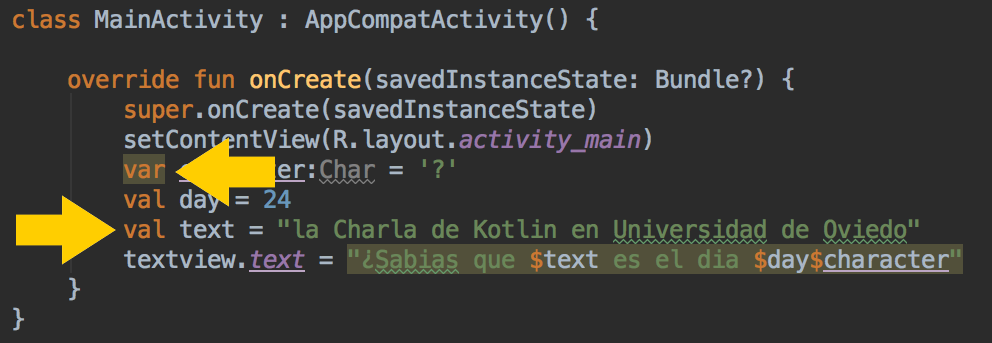
\includegraphics[width=\textwidth]{images/kotlin_vs_java/kotlin_val_var}
    \end{figure}
\end{frame}
%%%%%%%%%%%%%%%%

\begin{frame}{Sintaxis}{Getters \& Setters como properties}
    \begin{figure}[h]
    \centering
    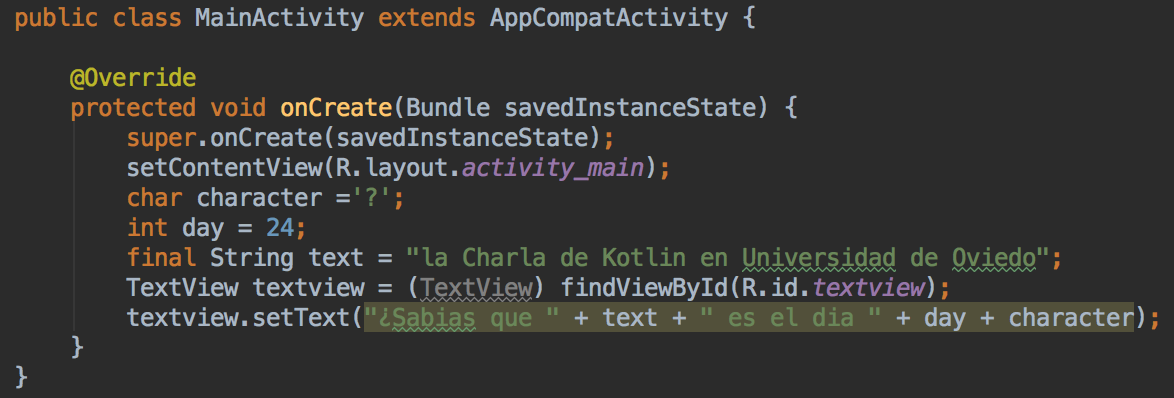
\includegraphics[width=\textwidth]{images/kotlin_vs_java/java_basic}
    \vspace{0pt}
    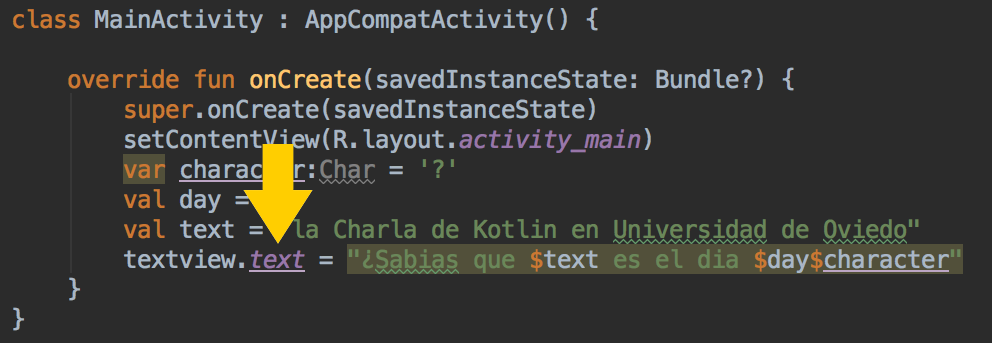
\includegraphics[width=\textwidth]{images/kotlin_vs_java/kotlin_properties}
    \end{figure}
\end{frame}
%%%%%%%%%%%%%%%%

\begin{frame}{Sintaxis}{String Templates}
    \begin{figure}[h]
    \centering
    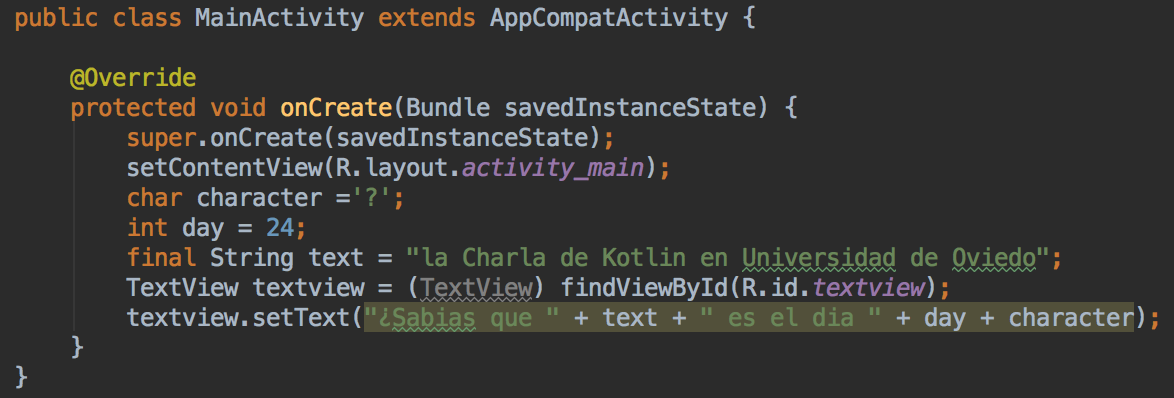
\includegraphics[width=\textwidth]{images/kotlin_vs_java/java_basic}
    \vspace{0pt}
    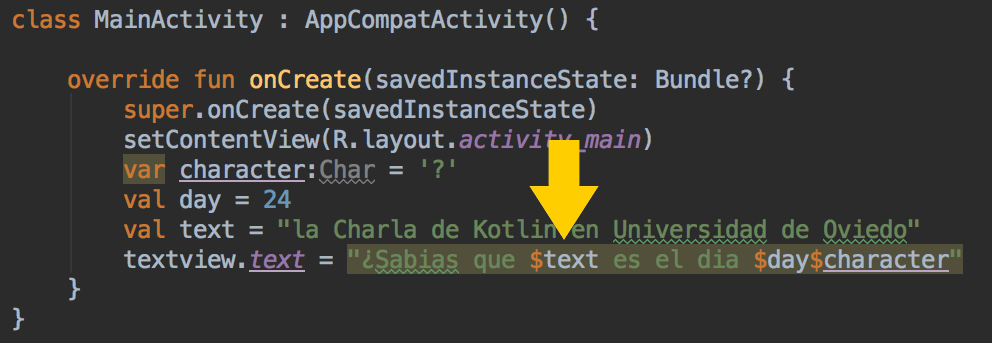
\includegraphics[width=\textwidth]{images/kotlin_vs_java/kotlin_string_templates}
    \end{figure}
\end{frame}
%%%%%%%%%%%%%%%%

\begin{frame}{Sintaxis}{new}
    \begin{figure}[h]
    \centering
    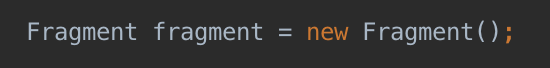
\includegraphics[width=\textwidth]{images/kotlin_vs_java/java_new}
    \vspace{0pt}
    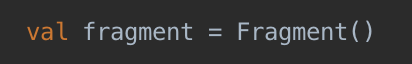
\includegraphics[width=\textwidth]{images/kotlin_vs_java/kotlin_new}
    \end{figure}
\end{frame}
%%%%%%%%%%%%%%%%

\begin{frame}{Sintaxis}{Singleton}
    \begin{figure}[h]
    \centering
    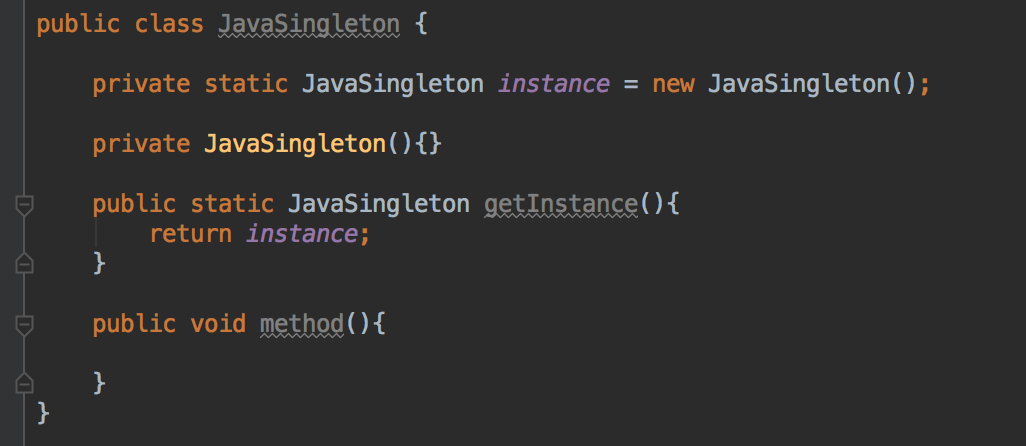
\includegraphics[width=\textwidth]{images/kotlin_vs_java/java_singleton}
    \end{figure}
\end{frame}
\begin{frame}{Sintaxis}{Singleton}
    \begin{figure}[h]
    \centering
    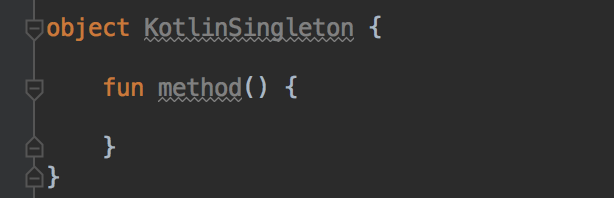
\includegraphics[width=\textwidth]{images/kotlin_vs_java/kotlin_singleton}
    \end{figure}
\end{frame}
\begin{frame}{Sintaxis}{Singleton}
    \begin{figure}[h]
    \centering
    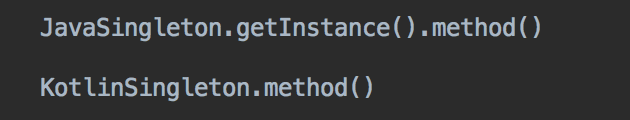
\includegraphics[width=\textwidth]{images/kotlin_vs_java/singleton_calls}
    \end{figure}
\end{frame}
%%%%%%%%%%%%%%%%

\begin{frame}{Sintaxis}{JavaBeans}
    \begin{figure}[h]
    \centering
    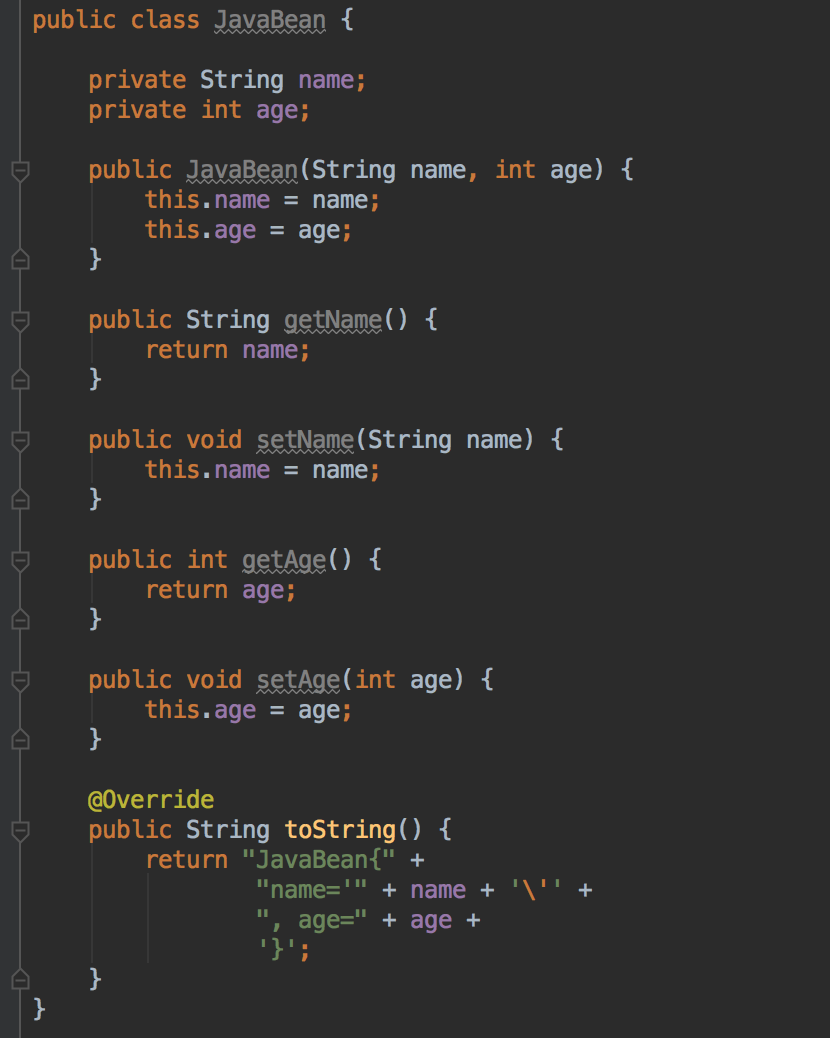
\includegraphics[width=0.6\textwidth]{images/kotlin_vs_java/java_bean}
    \end{figure}
\end{frame}
%%%%%%%%%%%%%%%%

\begin{frame}{Sintaxis}{Data classes}
    \begin{figure}[h]
    \centering
    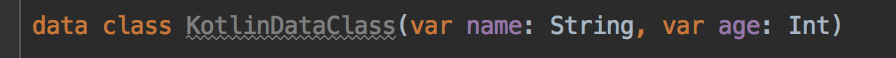
\includegraphics[width=\textwidth]{images/kotlin_vs_java/kotlin_data_class}
    \end{figure}
\end{frame}
%%%%%%%%%%%%%%%%

\subsection{Null}

\begin{frame}{Null}{Null Safety}
    \begin{figure}[h]
    \centering
    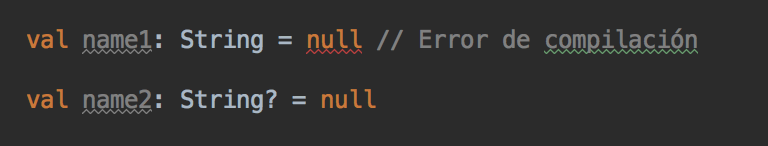
\includegraphics[width=\textwidth]{images/kotlin_vs_java/null_1}
    \end{figure}
\end{frame}
%%%%%%%%%%%%%%%%

\begin{frame}{Null}{Null Safety}
  \begin{block}{Llamadas seguras:}
    \begin{figure}[h]
    \centering
    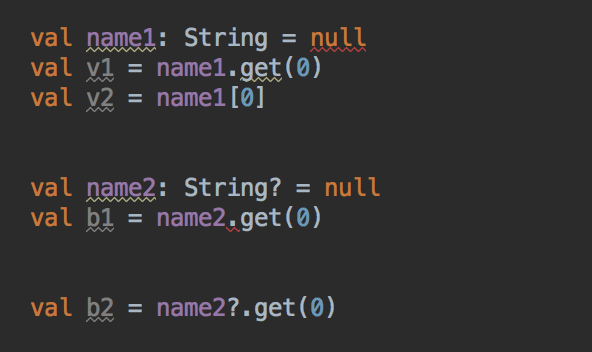
\includegraphics[width=\textwidth]{images/kotlin_vs_java/null_2}
    \end{figure}
     \end{block}
\end{frame}
%%%%%%%%%%%%%%%%

\begin{frame}{Null}{Null Safety}
  \begin{block}{Smart Cast:}
    \begin{figure}[h]
    \centering
    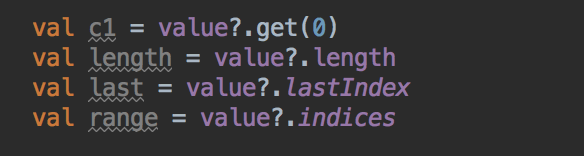
\includegraphics[width=\textwidth]{images/kotlin_vs_java/null_3}
    \vspace{0pt}
    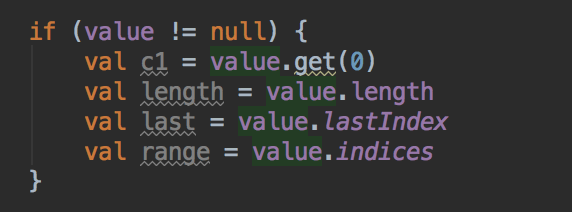
\includegraphics[width=\textwidth]{images/kotlin_vs_java/null_4}
    \end{figure}
     \end{block}
\end{frame}
%%%%%%%%%%%%%%%%

\begin{frame}{Null}{Null Safety}
  \begin{block}{Operador Elvis ?:}
    \begin{figure}[h]
    \centering
    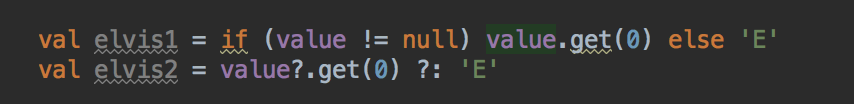
\includegraphics[width=\textwidth]{images/kotlin_vs_java/null_5}
    \end{figure}
  \end{block}
  \begin{block}{Operador !!}
    \begin{figure}[h]
    \centering
    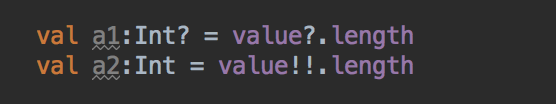
\includegraphics[width=\textwidth]{images/kotlin_vs_java/null_6}
    \end{figure}
  \end{block}
\end{frame}
%%%%%%%%%%%%%%%%

\begin{frame}{Null}{Null Safety}
  \begin{block}{Cast Seguro:}
    \begin{figure}[h]
    \centering
    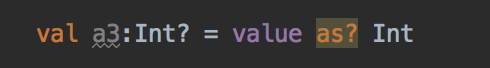
\includegraphics[width=\textwidth]{images/kotlin_vs_java/null_7}
    \end{figure}
  \end{block}
\end{frame}
%%%%%%%%%%%%%%%%





\subsection{Getter \& Setters}
\subsection{Delegados}
\subsection{Lazy \& lateinit}
\subsection{Parámetros opcionales}
\subsection{Lambdas}
\subsection{Métodos extensores}
